\documentclass[a4paper, 14pt, fleqn]{extarticle}
\usepackage{float}
\usepackage[justification=centering]{caption}
\usepackage{fefutitle}

\begin{document}
	\fefutitle{4}
	\pagebreak	

	\section{Введение}
		В данной лабораторной работе мне нужно решить и дать хар-ку линейных уравнений высших порядков, решить задачу Коши для уравнений 2-го порядка и
		найти коэффициент логистичекого уравнения.
	\pagebreak
	\section{Задание 1}
		\subsection{Постановка задачи}
			\noindent Для следующих линейных дифференциальных уравнений дать характеристику
					и найти общее решение:
		\begin{enumerate}
			\item \((\theta - 1)^4r^{\MakeUppercase{\romannumeral 4}} + 14(\theta - 1)^3r''' + 67(\theta - 1)^2r'' + 173(\theta - 1)r' + 320r = -5\sin^2{2\ln{(\theta - 1)}} \)
			\item \( \begin{aligned}[t] x''' - 8x'' + 21x' -20x &= -9e^{-2t}\cosh{3t}\cdot \sinh{3t} \cdot \cos{t} \cdot \sin{t} + \\ &+ (-10t+1)\cdot e^{3t}\cosh{4t} \end{aligned} \)	
			\item \(x^2y'' + xy' + y = 2\sin{\ln{x}}	 \)
			\item \( x(y''-y)\sin{x} + 2(xy' + y)\cos{x} + 2y'\sin{x} = e^x \)
			\item \( y'' + 4y = \sec{2x} \)
		\end{enumerate}
		\subsection{Решение}
			\noindent Поиск решения будет проводиться в системе компьютерной математики Wolfram Mathematica.
			\begin{enumerate}
				\item  \((\theta - 1)^4r^{\MakeUppercase{\romannumeral 4}} + 14(\theta - 1)^3r''' + 67(\theta - 1)^2r'' + 173(\theta - 1)r' + 320r = -5\sin^2{2\ln{(\theta - 1)}} \)

					\textit{Характеристика:} Линейное неоднородное приведенное дифференциальное уравнения четвертого порядка с переменными коэффициентами, приводится
										уравнению Эйлера 4 порядка заменой \( t = \theta -1 \) с характеристичекой неоднородностью
		
					\textit{Ответ:} \( \begin{aligned}[t] 768(\theta - 1)^4r &= C_1\sin\big(2\ln{(\theta - 1)}\big) + C_2\cos\big(2\ln{(\theta - 1)}\big) + \\&+ C_3\cos\big(4\ln{(\theta - 1)\big)} + C_4\sin{\big(4\ln{(\theta - 1)\big)}} +\\&+ 5\sin{\big(2\ln{(\theta - 1)}\big)} + 5\cos{\big(2\ln{(\theta - 1)}\big)} - 6   \end{aligned}\)

				\item \( \begin{aligned}[t] x''' - 8x'' + 21x' -20x &= -9e^{-2t}\cosh{3t}\cdot \sinh{3t} \cdot \cos{t} \cdot \sin{t} + \\ &+ (-10t+1)\cdot e^{3t}\cosh{4t} \end{aligned} \)

					\textit{Характеристика:} Линейное неоднородное приведенное дифференциальное уравнения третьего порядка с постоянными коэффициентами, характеристическая неоднородность
		
					\textit{Ответ:} \(\begin{aligned}[t] y &= C_1у^{4t}+e^{2t}(C_2\cos{2t} + C_3\sin{2t}) + Ae^{-2t} +\\ &+ e^{-2t}(B_1\cos{2t} + B_2\sin{2t} + Ee^{-8t} + e^{-8t}(F_1\cos{2t} +\\&+ F_2\sin{2t}) + Gxe^{4t} + e^{4t}(H_1\cos{2t} +H_2\sin{2t}) +\\&+ e^{7t}(J_1x+J_2) + e^{-t}(K_1x + K_2) \end{aligned}\)
				\pagebreak
				\item \(x^2y'' + xy' + y = 2\sin{\ln{x}} \)

					\textit{Характеристика:} Уравнение Эйлера второго порядка, характерестическая неоднородность после замены \( x = e^t \)
		
					\textit{Ответ:} \( y = C_1\cos{\ln{x}} + C_2\sin{\ln{x}} - \ln{x} \cdot \cos{\ln{x}}\)

				\item \( x(y''-y)\sin{x} + 2(xy' + y)\cos{x} + 2y'\sin{x} = e^x \)

					\textit{Характеристика:}  Линейное неоднородное неприведенное дифференциальное уравнения второго порядка с переменными коэффициентами
		
					\textit{Ответ:} \( xy = C_1\csc{x} + C_2x\csc{x} + e^x\csc{x} \)
 				\item \( y'' + 4y = \sec{2x} \)

					\textit{Характеристика:}  Линейное неоднородное приведенное дифференциальное уравнения второго порядка с постоянными коэффициентами, неоднородность общего вида
		
					\textit{Ответ:} \( 4y = C_1\cos{2x} + C_2\sin{2x} + 2x\sin{2x} + \cos{2x}\ln{\cos{2x}} \)

			\end{enumerate}

	\pagebreak
	\section{Задание 2}
		\subsection{Постановка задачи}
			\noindent Для заданных уравнений указать тип в простой форме. Найти общее решение. Найти частное решение, удовлетворяющее заданным условиям. Построить
					график решения:
			\begin{enumerate}
				\item \(2yy'' + y'^2 + y'^4 = 0;\;\; y(0) = 1,\; y'(0) = 2\)
				\item \(2yy'' = 4y'^2 + y'';\;\; y(0) = 0,\; y'(0) = -2\) 
			\end{enumerate}
		\subsection{Решение}
			\begin{enumerate}
				\item \(\begin{cases}
						2yy'' + y'^2 + y'^4 = 0, \\
						y(0) = 1, \\
						y'(0) = 2;
					\end{cases}\)

					\textit{Тип уравнения:} Общее уравнение несодержащее аргумента				

					\textit{Общее решение:} \( 2 (C_1y-1)^{\frac{3}{2}} + C_2 = 3C_1x \)
	
					\textit{Задача Коши:} \( (5y-4)^{\frac{3}{2}} - 1 = 15x \)

					\begin{figure}[H]
					   	\centering
					    	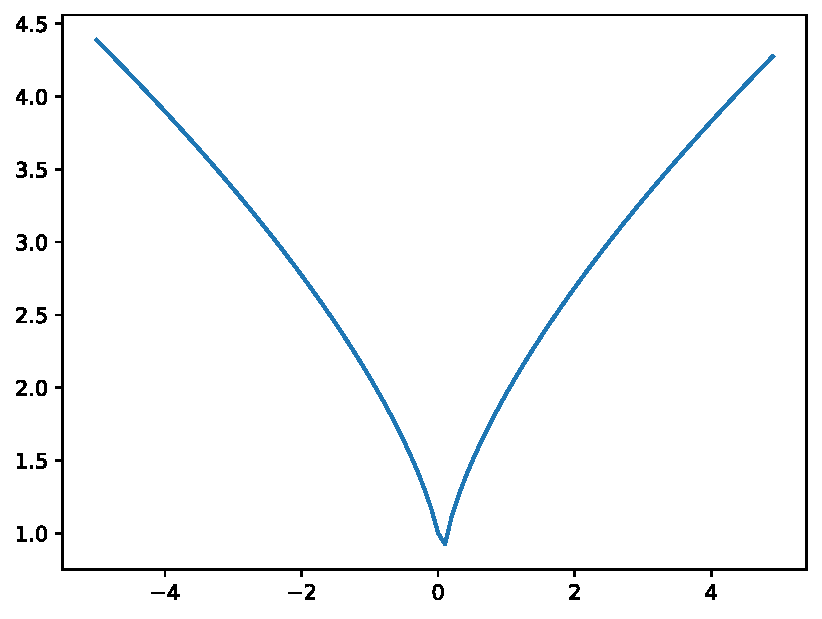
\includegraphics[width = .75\linewidth]{1.pdf}
						\caption[.] {График \( (5y-4)^{\frac{3}{2}} - 1 = 15x \)}
  					\end{figure}
			
				\item \(\begin{cases}
						r'' + 9r = 0,\\
						r(0) = \cos{4}, \\
						r'(0) = -3\sin{4};
					\end{cases}\)
					
					\textit{Тип уравнения:} Линейное однородное приведенное дифференциальное уравнения второго порядка с постоянными коэффициентами

					\textit{Общее решение:} \( r = C_1\cos{3\theta} + C_2\sin{3\theta} \)
	
					\textit{Задача Коши:} \( r = \cos{(3\theta + 4)} \)

					\begin{figure}[H]
					   	\centering
					    	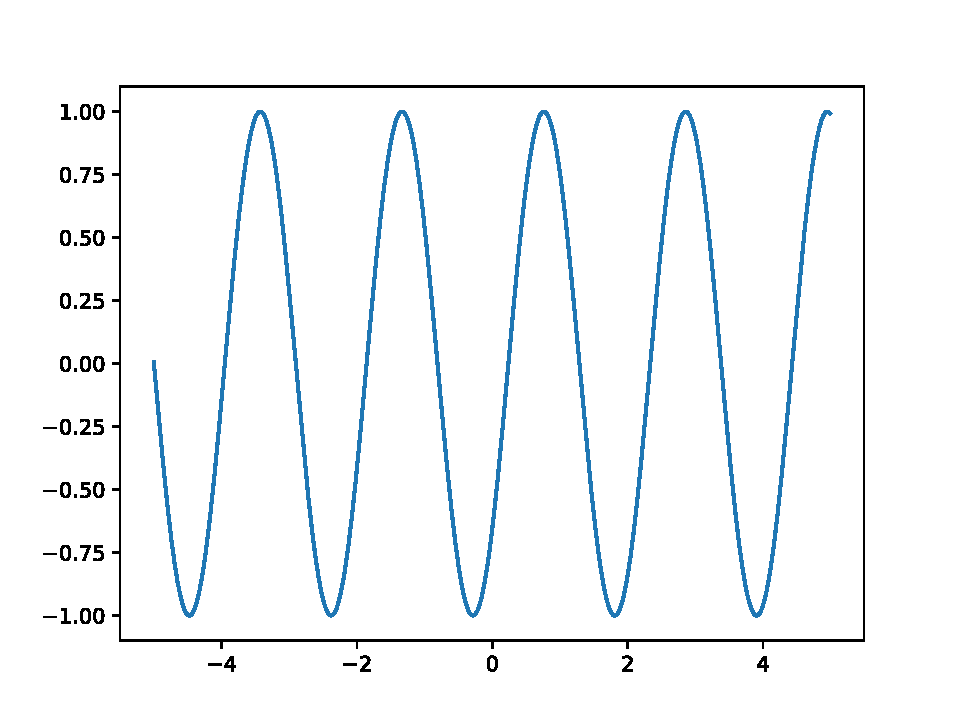
\includegraphics[width = .75\linewidth]{2.pdf}
						\caption[.] {График  \( r = \cos{(3\theta + 4)} \)}
  					\end{figure}
			\end{enumerate}

	\pagebreak
	\section{Заключение}
		\noindent Я решил 5 линейных уравнений высших порядков, 2 задачи Коши для уравнений 2-го порядка и аналитически нашёл коэффициент для логистического уравнения. Оформлял отчёт по работе в <<\TeX \:Live>>.
\end{document}	